\section{Characteristics of board games} \label{sec:boardgames_commonalities}

In this section we will analyse three different board games to identify and classify typical components of the board games. The purpose of this is to identify classic types of interactions and components in board games, so that we can focus on the central elements to implement in our platform. 

At the end we summarize the elements we've identified. The characteristical concepts of board games are described in subsection \ref{subsubsec:boardgame_concepts}, while the physical components common for board games can be found in subsection \ref{subsubsec:boardgame_components}. 

The three board games we've chosen is Lords of Waterdeep, Monopoly and Don't Panic. These are chosen to cover common, but different types of board games. Lords of Waterdeep is a classic Dungeons and Dragons game, making use of typical "advanced" board game dynamics, while Monopoly is a simpler common type of board game, employing many standard actions and elements. Don't Panic has been chosen as an existing hybrid board game.

\subsection{Monopoly}
Monopoly is a widely popular property trading game. Players acquire properties and money through chance cards, landing on property tiles and completing "laps" on the board. They charge each other money for the "use" (landing on) their land. Players lose by going "bankrupt", which is when their assets amount to less than 0 amount of money. The \textbf{winner is declared when} all other players are bankrupt.

\begin{figure}[ht]
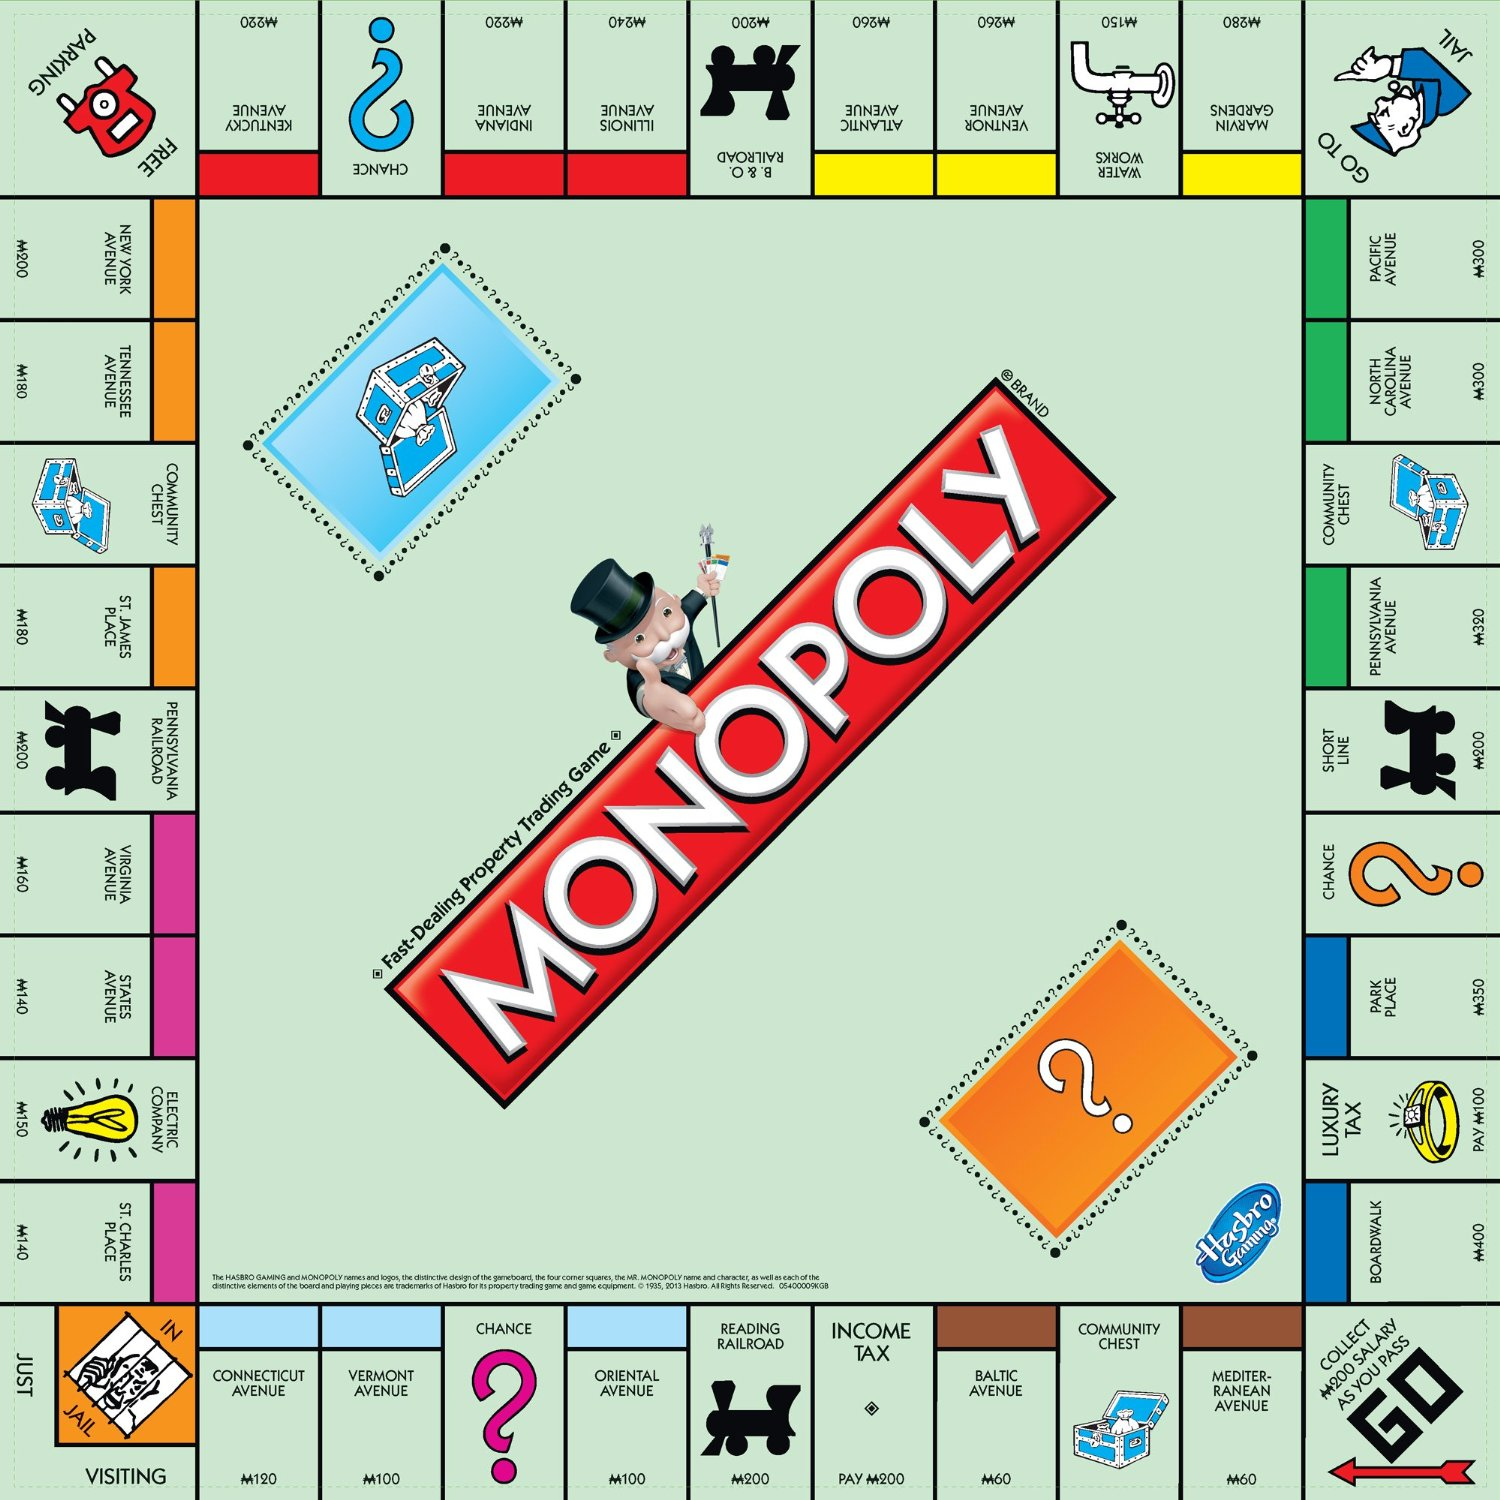
\includegraphics[width=12cm]{img/monopoly_board}
\centering
\caption{A version of Monopoly from Parker Brothers. Player pawns move from one to the next of the 40 tiles clockwise using two six sided dices.}
\label{fig:monopoly_board}
\end{figure}

The Monopoly \textbf{board} consists of roughly 40 discrete \textbf{tiles} as shown in figure \ref{fig:monopoly_board}. Each player has a \textbf{pawn} that represents them, which they move about the board with. The movement is determined by a roll of \textbf{dices}. Monopoly is \textbf{turn-based}, which means players take turn to throw the dices, moving their pawns, and completing a set of possible \textbf{actions} they can choose from, determined from the tile they land on. 

Each action usually involves buying, paying or exchanging  \textbf{resources} in form of money or stocks – which are placed in an inventory of each player. The inventory is a \textbf{private space} which contains the resources belonging to that player. Players starts the game with some initial resources in their inventory, but most are acquired during the game play. Resources are represented in form of two sorts of \textbf{informational tokens}: stocks and monopoly money. 

In short, the goal of the game is to maximize the acquisition of resources.

\subsection{Lords of Waterdeep} \label{subsec:LoW}
Lords of Waterdeep (LoW) is a \textbf{turn-based} game from the Dungeons and Dragons series, where players fight as a Lord in order to control a city. The goal of the game is to maximize the number of \textbf{points}. which are obtained mainly by completing quests. Quests are completed by obtaining a spesific combination of different adventureres in addition to a quest-card. 

In addition to quests and resources held by a player (marked red in figure \ref{fig:lords_board}), each player also is a spesific Lord (\textbf{Role}) which gives bonus points to certain quests for that player. LoW also include a type of cards called Intrigue, which can be used in various advantageous ways.

\begin{figure}[ht]
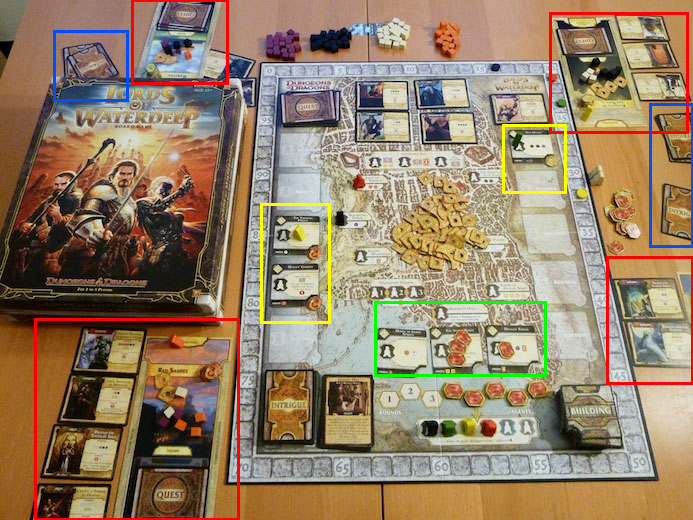
\includegraphics[width=12cm]{img/lords_board_marked}
\centering
\caption{Lords of Waterdeep. Players have multiple pawns and place them on available tiles as they please. New tiles (yellow) can be bought into the game allowing for a greater set of possible actions. Each player has both a visible (red) and hidden (blue) private space.}
\label{fig:lords_board}
\end{figure}

The Lord and Intrigue-cards are held in a \textbf{hidden private space}, a space that is not visible to other players other than the holder. Compared to games that doesn't have such dynamic, this hidden space introduces a new dimension to the game, as players hold different information.

LoW also make use of \textbf{rounds}. After all players have placed their pawns on the board, and actions has been completed, a round is over. All pawns are being put back into the inventory of each player, and points given by acquiring new tiles (buildings) are increased. After the fourth round, players are given an extra pawn, and the game ends after the eight round.

Another interesting component of LoW is its \textbf{dynamic board}. Of of the initial tiles can be used by players that wish to buy a new tile. The new tile will be an available in that and all the remaining rounds, and will reward the buyer upon usage.

\subsection{Don't Panic}
Don't Panic (DP) is a \textbf{cooperative} board game with different zones, where panic can emerge among "people" and spread to nearby zones. The players, unlike in Monopoly or LoW, work together in an effort to reduce panic. In DP, the players attempt to calm a situation down, and loses if the panic level goes beyond a certain threshold.

\begin{figure}[ht]
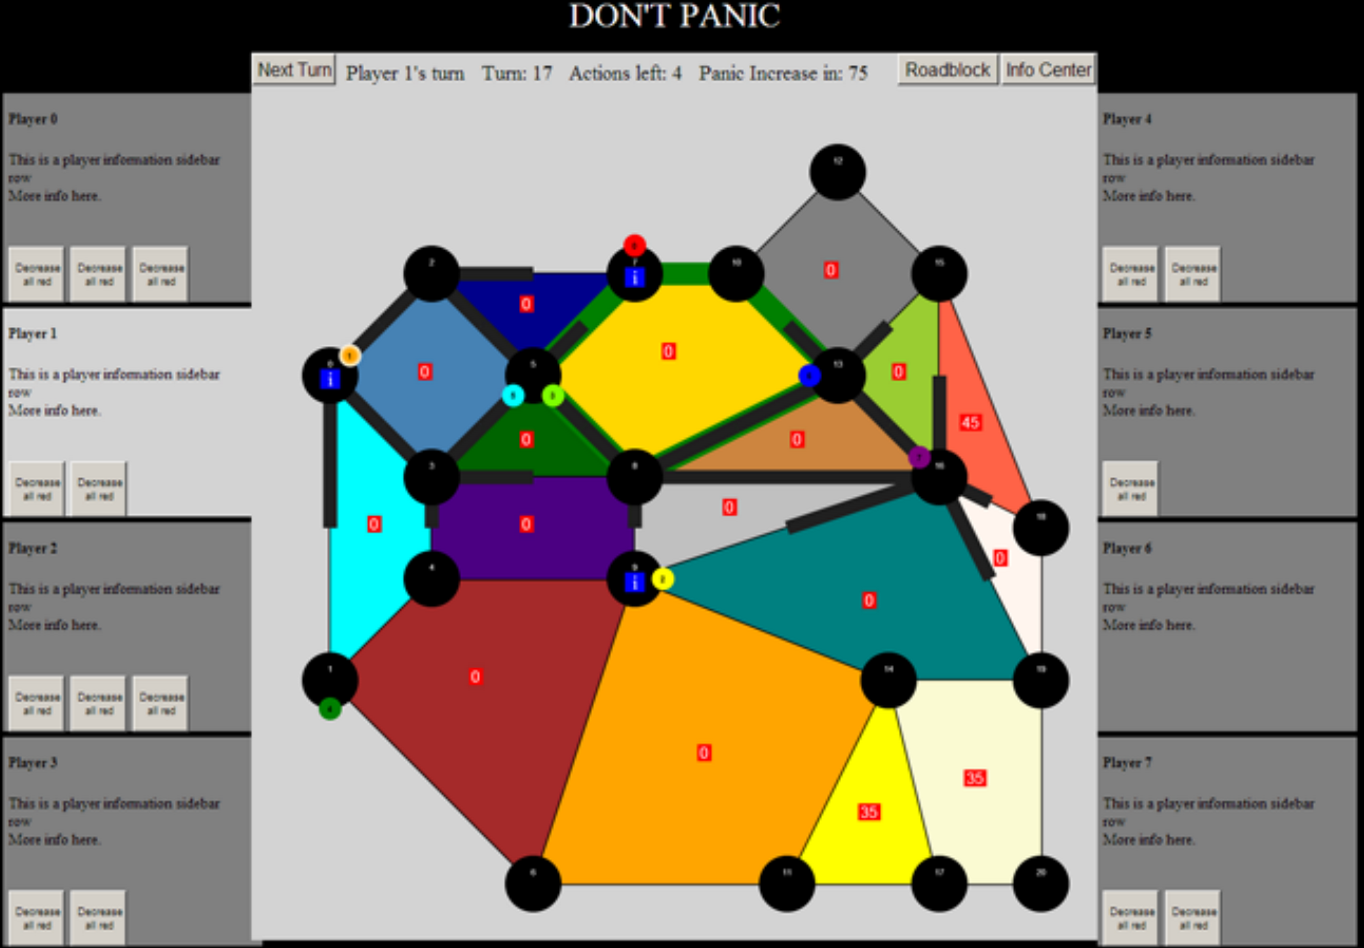
\includegraphics[width=12cm]{img/dont_panic_interface}
\centering
\caption{Digital version of Don't Panic. The map is divided into zones with a respective panic level. Player pawns locate themselves on the different nodes, and attempt to lower and contain the panic.}
\label{fig:dont_panic_board}
\end{figure}

Each player is presented by a pawn (colored circles in figure \ref{fig:dont_panic_board}) located on tiles (black nodes), and takes turn to draw 2 informational cards, 2 event cards and complete 4 "actions". Event cards are challenges which the players have to deal with on their turn, and can be resolved by "actions" or the use of informational cards. The informational cards are a form of resource that can (optionally) be used on a players turn. 

The 4 "actions" performed by players on each turn can be chosen from a set of actions containing movement of pawn, movement of people between zones, set up or remove road blocks to contain panic, as well as building an information center. Each player is also randomly given a role at the start of the game, which gives them an advantage on a spesific type of action. 

Once the game starts, a \textbf{timer} is initialized, counting down from a certain amount of minutes. Once the timer rings, panic levels are increased, and can spread between zones. This introduces a dimension of stress or hurry to the game, as playing faster gives an advantage.

\subsection{Summary: concepts} \label{subsubsec:boardgame_concepts}
\textbf{Players and Teams}: Board games are typically played in social settings with two or more players. In many board games such as Monopoly, each player is represented with a physical object called "pawn". In LoW, we saw that this is not the case, but rather had several agents that acted on behalf of the player.

Commonly, every player play each against other and is as such on team with only themselves, such as in Monopoly or Low. In other games, such as DP, several or all players can also play on teams with each other, fight common enemies even including the game itself.

\textbf{Roles and skills} are player-spesific properties that deviate from the standard rules of the game, and can give advantages or disadvantages in different aspects of the game. In DP, each player is assigned a Role by random, which gives them advantages in performing certain actions. For example, a driver can move more people out of paniced areas. Similarily in LoW, each player is assigned a Lord card (character) by random, which increases the points granted upon completing certain quests. LoW also has special quests that provide an advantage for the rest of the game (skill). For example, completing the quest "Quell Merchenary Uprising" will provide the player with two extra points for every other quest of the same type he or she completes.

\textbf{Public and private spaces}: Public and private spaces are the conceptual areas containing parts of the game that is interacted with by all or one of the players. Public spaces can be interacted with by all players, while each player has a private space that only that player can interact with. In Monopoly, question cards, dices and cards are a part of the public space, while money belong to the private spaces of each player.

\textbf{Hidden private space}, is the a private space that is not visible for other players. For example a hidden hand contains cards that are visible only to the holder of the cards. For example in LoW your Intrigue cards (uncommon advantageous actions you can perform) is hidden from other players. 

\textbf{Themes} provide a background story and explain the motivation and goal for the players. Both Monopoly, LoW and DP have themes that help relate the game to real world concepts and provide some story that can help players immerse them selves in the games. This is unlike games as Poker or Tic Tac Toe.

\textbf{Events} are special parts of the game that often go outside the normal flow of the game. In Monopoly, one of the tiles will send you to "jail". This includes a movement of the pawn that is not based on dices like the rest of the game, and gives an exception to the dice rolling and movement in the next turns. An event is also triggered when drawing question cards: winning the lottery or having to repair your houses go outside the normal flow of the game. In LoW, playing Intrigue cards will trigger events, allowing for players to take resources from others or imposing a mandatory quest upon other players. And in DP, Event Cards and playing Informational Cards can be categorized as events. Events are typically unpredictable, either by being in a shuffled deck of cards or played from a hidden private space.

\textbf{Resources} are assets belonging to a player. In Monopoly, the resources are Stocks, Money and Houses. Player controlled events, such as the Get Out of Jail Free Card (Monopoly) or Intrigue card (LoW) can also be considered resources. Resources are often made physical through Indicator Tokens (see \ref{subsubsec:boardgame_components}).

\textbf{Turns and actions}: In turn-based games each player takes turn to complete some actions, before the next person plays his turn. Each turn usually involves a scripted set of actions. In Monopoly, you must always roll two dices and move your pawn that amount of tiles. This is a mandatory action. The tile determines the next set of actions you can perform. Either 1) pay the owner rent (mandatory), if the tile is currently owned by anther player, 2) buy the stock (optional) if the tile is for sale, 3) draw a card and complete it's action (mandatory) if landing on a question-tile. In other words, turns are sets of actions, where each action can either be mandatory or optional, that can have a precondition, i.e. do this if that, and can be ordered, i.e. done in a speific order.

\textbf{Rounds} is a concept that some event or set of events will incur, usually that sets back the game in some way, after some critiera is met. In LoW, actions is performed via agents, which is "spent" once put on the board. When all agent actions are exhausted, the round is over, and agents are put back into their respective players private space so that they can perform actions on behalf of the player again. In DP, one can interpret the time between each alarm as a round. Once the round is over, panic is increased and potentially spread.

\textbf{Rules} tell us the possible interactions between game components: Which actions is involved in a turn? When is a round over? How can your pawn move around the board? When is a winner declared, or a player out of the game? Rules explicitly define the starting conditions upon starting the game, and are a central part of all games, as they dictate the flow of the game and define the bounderies of them.

\subsection{Summary: Physical components} \label{subsubsec:boardgame_components}

\begin{figure}[ht]
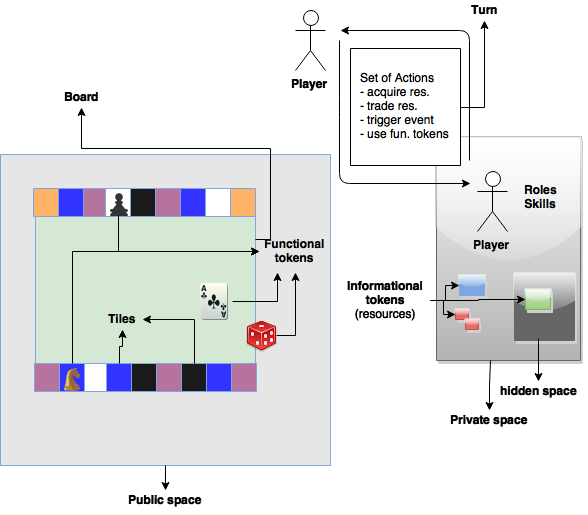
\includegraphics[width=12cm]{img/board_games_components}
\centering
\caption{Common components of board games. Board with tiles and functional tokens as a part of the public space, while informational tokens (resources) as part of each players private space, potentially hidden from view from other players. The game is progressed by players taking turn to acquire and trade resources, triggering events and interacting with functional tokens.}
\label{fig:board_games_components}
\end{figure}


\textbf{Board} is the surface used to play a board game. Most games have a unchanging board (Monopoly), while some have a modular board with varying layout in each session or while the game is played (LoW). The board consists of tiles and placeholders for other assets.

\textbf{Tiles} are discrete locations on the board. Which tile a player is located on, usually determines which set of \emph{actions} the player can perform. In Monopoly for example, a stock can only be bought when the the pawn is located on that spesific tile. In Don't Panic, it didn't determine which actions one could perform, but rather which part of the city the player could perform his actions upon. In some games, such as Monopoly and DP, movement is only allowed over adjecent tiles.

\textbf{Indicator tokens}, e.g. Gold, Wood, Stone, Gas, Money, Points, Stocks and Houses help keeping track of an informational aspect in the game. In Monopoly, the paper money is simply an indicator of how much resources owns, and stocks an indicator of the lots owner. It serves its purpose by holding some information, and as such simplifying the amount of information players have to remember and keep track of themselves.

These are simple tokens, as they are only representatational of some game information, and does not change the game state or provide interactive functionality like randomness. Such tokens can easily be replaced by a number value or position on a screen, as they are not interacted with other than changing owner.

\textbf{Functional tokens}, e.g. dice, cards and pawns play an active part in how the game unfolds. For example, a dice in provides randomness as a functionality to the player, while the timer in DP provide an aspect of time or hurry. Cards are the most common functional tokens, which can provide many types of events and exceptions to the standard flow of the game, as well as provide randomness through being shuffled and used in a drawable deck.

These tokens change the state of the game by opening or closing certain actions and aspects for players. Each of these tokens have a specialized functionality, and can not be implemented as generally as indicator tokens.

\newpage
